\documentclass[a4paper,10pt]{article}
\usepackage[utf8]{inputenc}
\usepackage{amsmath}
\usepackage{fullpage}
\usepackage{hyperref}
\usepackage{graphicx}
\usepackage{listings}
\usepackage{color}

\definecolor{mygreen}{rgb}{0,0.6,0}
\definecolor{mygray}{rgb}{0.5,0.5,0.5}
\definecolor{mymauve}{rgb}{0.58,0,0.82}

\lstset{ 
  backgroundcolor=\color{white},   % choose the background color; you must add \usepackage{color} or \usepackage{xcolor}; should come as last argument
  basicstyle=\footnotesize,        % the size of the fonts that are used for the code
  breakatwhitespace=false,         % sets if automatic breaks should only happen at whitespace
  breaklines=true,                 % sets automatic line breaking
  captionpos=b,                    % sets the caption-position to bottom
  commentstyle=\color{mygreen},    % comment style
  deletekeywords={...},            % if you want to delete keywords from the given language
  escapeinside={\%*}{*)},          % if you want to add LaTeX within your code
  extendedchars=true,              % lets you use non-ASCII characters; for 8-bits encodings only, does not work with UTF-8
  firstnumber=1,                   % start line enumeration with line 1000
  frame=single,	                   % adds a frame around the code
  keepspaces=true,                 % keeps spaces in text, useful for keeping indentation of code (possibly needs columns=flexible)
  keywordstyle=\color{blue},       % keyword style
  language=Python,                 % the language of the code
  morekeywords={*,...},            % if you want to add more keywords to the set
  numbers=left,                    % where to put the line-numbers; possible values are (none, left, right)
  numbersep=5pt,                   % how far the line-numbers are from the code
  numberstyle=\tiny\color{mygray}, % the style that is used for the line-numbers
  rulecolor=\color{black},         % if not set, the frame-color may be changed on line-breaks within not-black text (e.g. comments (green here))
  showspaces=false,                % show spaces everywhere adding particular underscores; it overrides 'showstringspaces'
  showstringspaces=false,          % underline spaces within strings only
  showtabs=false,                  % show tabs within strings adding particular underscores
  stepnumber=1,                    % the step between two line-numbers. If it's 1, each line will be numbered
  stringstyle=\color{mymauve},     % string literal style
  tabsize=4,	                   % sets default tabsize to 2 spaces
  title=\lstname                   % show the filename of files included with \lstinputlisting; also try caption instead of title
}


%opening
\title{NUR Assignment 1}
\author{Christiaan van Buchem - s1587064}

\begin{document}

\maketitle

\begin{abstract}
 In this document an example solution template is given for the exercises in the 
 course Numerical recipes for astrophysics.
\end{abstract}

\section{Exercise 1}

For this first exercise we had to write our own Poisson probability distribution function and random number generator. The output of the Poisson function can be seen in the printed text (see below) and the tests for the rng can be found in \ref{fig:fig1.1} and \ref{fig:fig1.2}.

\subsection{Scripts}
The functions that I wrote for this exercise can be found in: 
\lstinputlisting{NR_a1_1_utils.py}

The commands used to retrieve the desired results are given by:
\lstinputlisting{NR_a1_1_main.py}

The result of the given script is given by:
\lstinputlisting{NR_a1_1_main.txt}


\begin{figure}[h!]
  \centering
  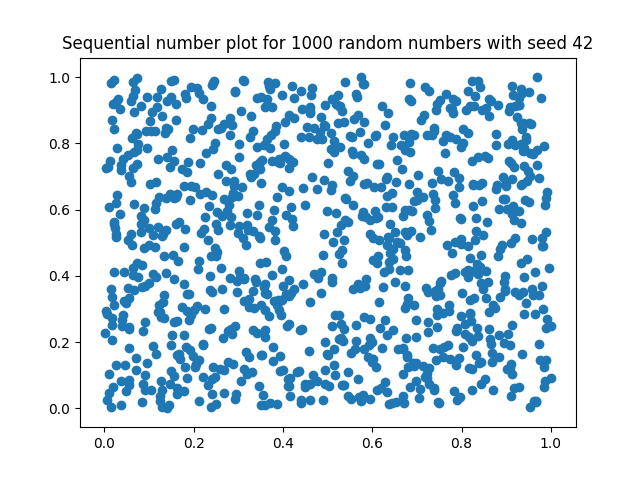
\includegraphics[width=0.9\linewidth]{./plots/1_b_1.png}
  \caption{In this figure we can see that it appears that the random number generator is producing numbers without a certain preference.}
  \label{fig:fig1.1}
\end{figure}

\begin{figure}[h!]
  \centering
  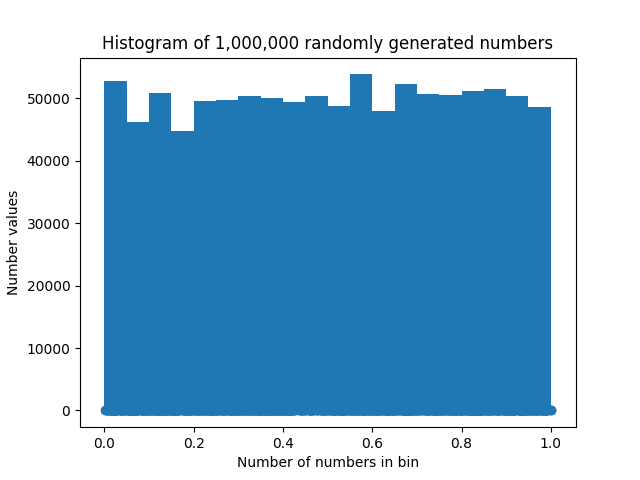
\includegraphics[width=0.9\linewidth]{./plots/1_b_2.png}
  \caption{This histogram places the random number generator under a sharper knife, allowing us to see that there are some fluctuations between the bins. Overal it appears to be quite unbiased.}
  \label{fig:fig1.2}
\end{figure}
 
\section{Exercise 2}

For this section of the assignment we were asked to write a variety of different functions in order to probe the given probability function $n(x)$. These will be discussed per sub-question:

\subsection{Write a numerical integrator}

In order to accomplish this task I wrote an integrator that uses Romberg's algorithm in order to numerically integrate a given function from a to b.  

The output values are found in the print statement produced by the script.

\subsection{Make a log-log plot and interpolate the given values}

For this I used a linear-interpolator due to the fact that at first glance these values follow a linear trend in log-log space. Due to having too little time I did not manage to alter my interpolator to also work in log-space. For this reason the interpolated function systematically overshoots the fit one would expect. We can see this well in \ref{fig:fig2.1}. 

\begin{figure}[h!]
  \centering
  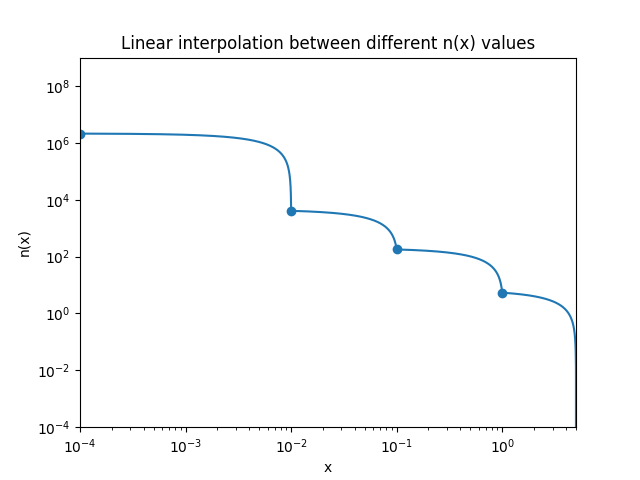
\includegraphics[width=0.9\linewidth]{./plots/2_b.png}
  \caption{Here we see the way in which a linear interpolator overshoots the expected function when used in log-space.}
  \label{fig:fig2.1}
\end{figure}

\subsection{Numerically calculate $dn(x)/dx$ at $x=b$}

For this task I wrote an algorithm that numerically differentiates using Ridder's method. The analytic and calculated numerical value can be found in the print statement.

\subsection{Generate 3D satellite positions}

In order to generate this distribution I used the rejection sampling method. The positions generated using this method can be found in the print statement. 

\subsection{Repeart (d) for 1000 haloes each containing 100 satellites} 

The histogram generated for this task can be found in \ref{fig:fig2.2}. It appears that the generated galaxies match the distribution fairly well. It is only really lacking at the lower end of the distribution. 

\begin{figure}[h!]
  \centering
  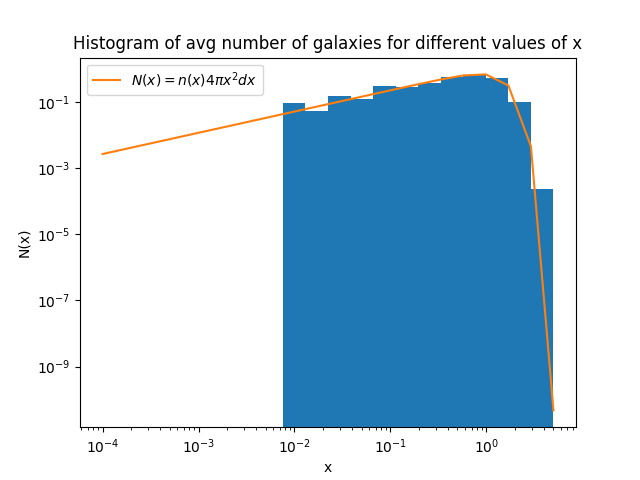
\includegraphics[width=0.9\linewidth]{./plots/2_e.png}
  \caption{Histogram of number of satellites in each bin with over-plotted probability. Note the discrepancy at the lower end of the distribution.}
  \label{fig:fig2.2}
\end{figure}

\subsection{Write a root-finding algorithm}

The method I used in order to find these roots is the Newton-Raphson method. This is because the false-position method and Secant method appeared not to be able to converge for this function. The values of the roots are given in the print output. 

\subsection{Take the bin from e containing the largest number of galaxies. Using sorting calculate the median, 16th and 84th percentile for this bin and output the values and plot the histogram}

The calculated values for the median, 16th and 84th percentile can be found in the print statement. 

The histogram produced for this task can be found in \ref{fig:fig2.3}.

\begin{figure}[h!]
  \centering
  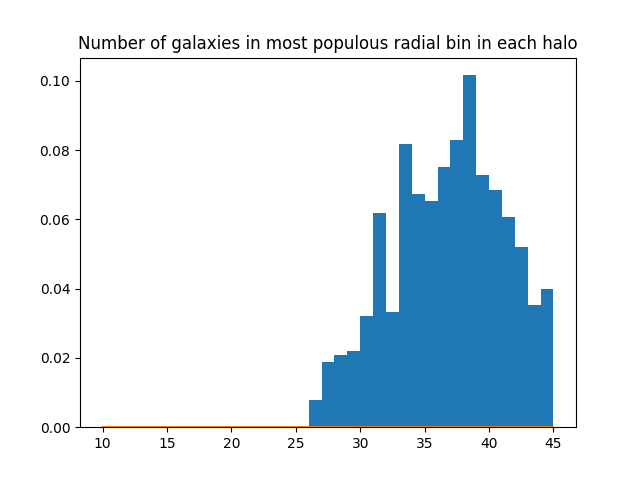
\includegraphics[width=0.9\linewidth]{./plots/2_g.png}
  \caption{Number of galaxies in most populous radial bin in each halo. Note that the Poisson distribution is most likely calculated wrongly.}
  \label{fig:fig2.3}
\end{figure}

As you can (barely) see, the Poisson distribution does not match the histogram. This however is most likely due to a mistake in my Poisson distribution function.

\subsection{Write an interpolator that gives values of a for different a,b,c}

In order to accomplish this task I wrote a function for a trilinear-interpolator. The values I tested it with and the resulting A value can be found in the print statement.

\subsection{Scripts}

The functions that I wrote for this exercise can be found in: 
\lstinputlisting{NR_a1_2_utils.py}

The commands used to retrieve the desired results are given by:
\lstinputlisting{NR_a1_2_main.py}

The result of the given script is given by:
\lstinputlisting{NR_a1_2_main.txt}

\section{Exercise 3}

For the third exercise we were to work with the data given to us. We also had to write down the log-likelihood corresponding to a set of random realizations of the satellite profile. This is give by:

\begin{equation}
\log L = N \log(A(a,b,c) + (a-1) (\sum\limits_{i=1}^{N-1} \log(x_i) - N \log(b)) + \sum\limits_{i=1}^{N-1} -(\frac{x_i}{b})^c
\end{equation}

\subsection{Find the a,b,c that maximize this likelihood}

In order to accomplish this task I decided to find the minimum of the $-log$ likelihood. For this I wrote an algorithm that uses the Simplex (also known as the Nelder-Mead method). This function worked well for the test function that I gave it, but I did not manage to keep it within the range given for a,b,c. Given a bit more time, this function would most likely have worked. In order to test it I used the data found in $satgals_m15$.
\subsection{Write an interpolator fora,bandcas a function of halo mass,orfit a function to each.}

I did not manage to accomplish this task due to time constraints. 

\subsection{Scripts}

The functions that I wrote for this exercise can be found in: 
\lstinputlisting{NR_a1_3_utils.py}

The commands used to retrieve the desired results are given by:
\lstinputlisting{NR_a1_3_main.py}

The result of the given script is given by:
\lstinputlisting{NR_a1_3_main.txt}

\end{document}
